\chapter{Introduzione}
\label{chap:1}

\section{Contestualizzazione}
\label{sec:Contestualizzazione}

\subsection{Evoluzione delle applicazioni web}
Inizialmente le applicazioni web erano costituite da semplici pagine statiche contenenti testo e immagini.
Col passare degli anni, grazie all'adozione di JavaScript e di librerie e framework correlati, hanno progressivamente acquisito un carattere più dinamico, con l'introduzione di livelli crescenti di interattività. 
Un cambiamento significativo in tal senso, è avvenuto con l'avvento delle \textbf{Single Page Application (SPA)} e di \textbf{AJAX}.
Tale combinazione, ha infatti introdotto un nuovo paradigma di sviluppo, in cui l'intera appplicazione viene caricata una sola volta e le successive interazioni con l'utente avvengono grazie al caricamento dinamico di contenuti e dati provenienti da un web server, eliminando così l'attesa nel caricamento di una nuova pagina e favorendo l'esperienza d'uso.
\\Parallelamente, la complessità delle funzionalità offerte è cresciuta in modo esponenziale, spaziando da applicazioni di grafica 3D, a simulatori, ad applicazioni di modifica di documenti, immagini e video.
Oggi, è sempre più comune incontrare siti web in grado di gestire complesse operazioni in tempi rapidi, assicurando così quell'interattività alla quale ormai siamo abituati. 
Tuttavia questo progresso è stato accompagnato da un aumento del numero di richieste effettuate in rete e dall'utilizzo intensivo di risorse computazionali, sia lato cliente, che lato servitore.
\begin{figure}
        \begin{center}
                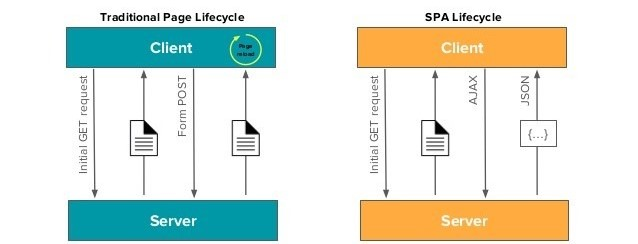
\includegraphics[width=0.9\columnwidth]{images/spa.jpg}
        \end{center}
        \caption{Differenza nel tipo di richieste tra SPA e MPA.}
        \label{fig:spa}
\end{figure}
        
\subsection{Importanza dell'ottimizzazione}
Ad oggi, l'ottimizzazione delle prestazioni è quindi diventata un aspetto cruciale nello sviluppo di applicazioni web.
Gli utenti si aspettano interazioni con bassa latenza, caricamenti rapidi e risposte immediate.
Questa esigenza mette in risalto l'importanza di bilanciare l'aggiunta di funzionalità sofisticate, con l'offerta di una \emph{User Experience} ottimale.
\\I tempi di caricamento prolungati possono portare a un alto tasso di abbandono delle pagine, riducendo l'opportunità di coinvolgere nuovi utenti.
Inoltre, con l'aumentare dell'utilizzo di dispositivi mobili e di conseguenza, di connessioni instabili, l'ottimizzazione diventa ancor più critica per assicurare un'esperienza coerente su diverse piattaforme e condizioni di rete.
Tutto ciò non riguarda solo il lato client, ma coinvolge anche il lato server. 
Un carico eccessivo sui server può influire negativamente sulla scalabilità, causando ritardi nelle risposte e possibili interruzioni del servizio.
L'ottimizzazione deve quindi coinvolgere tutti gli aspetti dell'architettura delle applicazioni web.
\\Nell'implementare ottimizzazioni, sono nati varie soluzioni interessanti. Ad esempio, per gestire task che svolgono molte operazioni di Input/Output si è distinto \textbf{Node.js}, mentre per quanto riguardo l'esecuzione di attività che sfruttano molto la CPU è emerso \textbf{WebAssembly(Wasm)}, in sinergia con l'interfaccia di sistema \textbf{WebAssembly System Interface (WASI)}.


\newpage
\section{Motivazioni e Obiettivi}
\label{sec:Obiettivi}
La crescente complessità delle applicazioni web e l'esigenza di offrire agli utenti esperienze interattive sempre più coinvolgenti hanno portato l'ambito dello sviluppo web a una svolta significativa.
Le aspettative degli utenti si sono evolute verso applicazioni che offrano prestazioni reattive, interattività immediata e funzionalità avanzate.
\\È proprio questo insieme di aspettative a essere alla base delle motivazioni che hanno guidato la scelta del tema di questa tesi di laurea.
\\In particolare, la presente ricerca, si propone di confrontare in modo dettagliato, due differenti approcci di sviluppo per un'applicazione con funzionalità fortemente CPU-Intensive.
\subsection{Tipologia di applicazione}
Per tale confronto, si è optato per una web-app che utilizzi alcune tecniche di elaborazione di immagini.
In particolare, all'utente sarà consentito eseguire l'upload di immagini su un server e indicare una serie di modifiche da apportare (ad esempio "ridimensionamento del 50\%"). Tale server le eseguirà secondo i parametri ricevuti e infine restituirà al cliente le immagini modificate.
\\Non verrà esplorato in modo approfondito il campo dell'elaborazione digitale di immagini, ma ci si limiterà all'implementazione di funzionalità usate spesso da utenti comuni, come ad esempio, ridimensionamento, rotazione, aumento/diminuzione di luminosità e contrasto e altre che verranno specificate nel capitolo \ref{chap:3}.
\\Tale tipologia di applicazione, si sposa bene per lo scopo finale della tesi: valutare come due aprrocci (e due linguaggi) piuttosto differenti, ma sempre più diffusi al giorno d'oggi, risolvano il problema di un'applicazione web che svolga operazioni dall'alto costo computazionale.
\subsection{Metodologie confrontate}
Le due modalità di sviluppo in esame riguarderanno l'utilizzo delle tecnologie JavaScript e WebAssembly server-side e quindi rispettivamente del runtime environment Node.js e del linguaggio di programmazione Rust in combinazione con WebAssembly System Interface. 
\\La scelta di Node.js deriva dalla sua crescente popolarità dovuta all'utilizzo del linguaggio JavaScript, dall'approccio asincrono nella gestione delle richieste e dalla sua ottima scalabilità per applicazioni fortemente File-System-Intensive.
Per quanto riguarda la seconda tecnologia si è invece optato per Rust, in quanto consente sia la scrittura di moduli che succesivamente compilabili in WebAssembly, sia il loro utilizzo efficiente all'interno del codice, mantenendo in questo modo un'ottima coerenza e risultando, teoricamente, una buona scelta per lo sviluppo di applicazioni computazionalmente complesse. 
\begin{figure}
        \begin{center}
                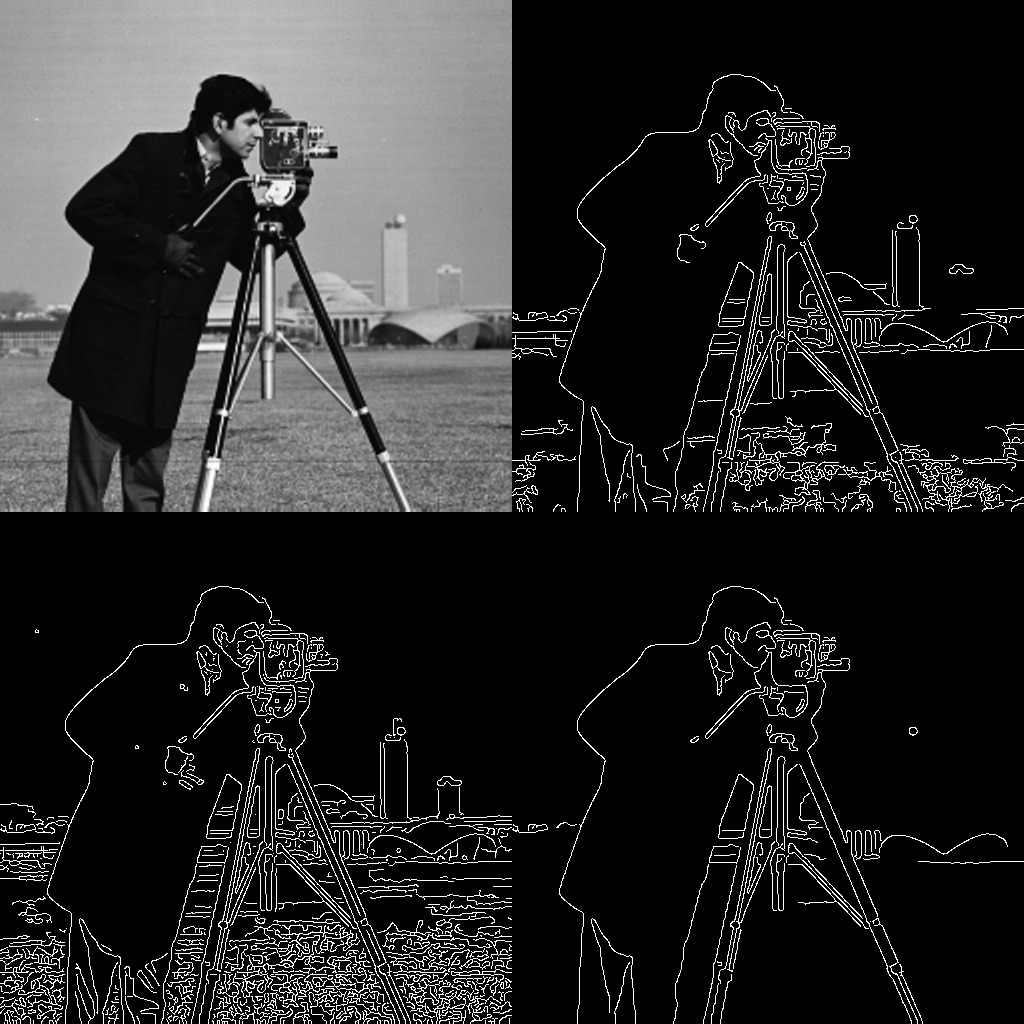
\includegraphics[width=0.7\columnwidth]{images/imageProc.jpg}
        \end{center}
        \caption{Il campo dell'elaborazione digitale di immagini è molto ampio e sarebbe possibile integrare anche operazioni avanzate (edge detection, pattern recognition etc.), che richiederebbero risorse computazionali molto elevate. Per lo scopo di questa tesi ci si limiterà a elaborazioni più semplici, ma in ogni caso rilevanti e sufficienti a mettere alla prova la CPU.}
        \label{fig:imageProc}
\end{figure} 
\subsection{Analisi Comparativa delle Tecnologie}
Un elemento iniziale di questa ricerca sarà un analisi dettagliata delle tecnologie prese in esame. 
Inizialmente, nel capitolo \ref{chap:2}, verrà svolta un'analisi comparativa delle due tecnologie, presentando i vantaggi e gli svantaggi teorici di entrambe.
\\Sarà infatti fondamentale comprendere come ciascuna affronti la complessità legata ad operazioni I/O-intensive e CPU-intensive, per valutare nel modo più opportuno i risultati ottenuti in fase di test e benchmark dell'applicazione sviluppata.
\\Si procederà poi ad illustrare in modo approfondito il funzionamento delle API sfruttate. Verranno analizzate le peculiarità del linguaggio Rust che lo rendono adatto ad applicazioni ad alta intensità computazionale, nonchè l'efficacia di WebAssembly nell'esecuzione di codice di basso livello con prestazioni paragonabili a quelle dei linguaggi nativi.
\\Nel contempo si analizzerà anche la metodologia basata su Node.js, concentrandosi sull'efficienza e la flessibilità che questo ambiente di esecuzione JavaScript può offrire in ambito web.
\\Si proseguirà affrontando un'analisi dettagliata delle prestazioni di ciascuna tecnologia, evidenziando scenari in cui una risulti più vantaggiosa. Questo approfondimento sarà alla base delle successive valutazioni sulle prestazioni delle applicazioni sviluppate con i due metodi presi in esame.
\begin{figure}
        \centering
        \begin{minipage}{0.40\textwidth}
            \centering
            
\includegraphics[width=0.9\textwidth]{images/rustwasm.jpg} 
            \caption{Rust e Wasm}
        \end{minipage}\hfill
        \begin{minipage}{0.40\textwidth}
            \centering
            
\includegraphics[width=0.9\textwidth]{images/node.png} 
            \caption{Node.js}
        \end{minipage}
    \end{figure}

\subsection{Valutazione dell'Impatto di Wasm}
WebAssembly, in particolare, è emerso come un'innovazione cruciale nel mondo dello sviluppo web.
Consentendo l'esecuzione di codice a basso livello con prestazioni paragonabili a quelle dei linguaggi nativi, Wasm offre la possibilità di ottenere prestazioni elevate all'interno di un ambiente browser-based.
\\Parallelamente, WebAssembly System Interface (WASI) gioca un ruolo chiave nell'estendere il potenziale di WebAssembly. WASI fornisce un'interfaccia standardizzata per l'accesso a risorse di sistema, consentendo alle applicazioni di interagire con l'ambiente circostante in modo controllato e sicuro. Tale capacità è particolarmente rilevante nell'ambito delle applicazioni web CPU-intensive, in quanto consente di accedere, in maniera efficiente, alle risorse di sistema necessarie per eseguire complesse operazioni di calcolo e manipolazione dei dati.

\subsection{Obiettivi}
Si intende esplorare le opportunità offerte dalle tecnologie enunciate sopra, nell'ottica di un'ottimizzazione delle prestazioni.
In questo contesto l'obiettivo sarà quello di comprendere i benefici specifici di ciascun approccio, individuando le circostanze in cui uno dei due possa risultare vantaggioso in termini di efficienza computazionale e reattività. Inoltre si vorrà sottolineare l'importanza, sin dalla fase di progettazione, di un'attenta analisi per determinare se un'applicazione sia maggiormente orientata al calcolo intensivo o all'uso massiccio del File System. 
Per raggiungere in maniera efficace e misurabile gli obiettivi, verrà fatta un'analisi approfondita delle performance e delle prestazioni delle due applicazioni sviluppate.

\newpage
\section{Trend di evoluzione del web}
\label{sec:Trend}
\subsection{Paradigmi di Sviluppo Moderni}

\subsection{Esperienze Utente Migliorate ?}



\section{Struttura della tesi}
\label{sec:struttura}

This is a reference to a chapter \ref{chap:1}. This is a reference to a figure \ref{fig:doge}. This is a reference to some code \ref{lst:hello}. This is a citation \cite{famous:paper}.

\lstinputlisting[label=lst:hello, firstline=2, lastline=4, caption={I directly included a portion of a file}]{code/hello.py}

\begin{lstlisting}[language=Java, label=lst:java, caption={Some code in another language than the default one}]
public void prepare(AClass foo) {
        AnotherClass bar = new AnotherClass(foo)
}
\end{lstlisting}


\begin{figure}
\begin{center}

\includegraphics[width=0.3\columnwidth]{images/doge.png}
\end{center}
\caption{This is not a figure. It's a caption.}
\label{fig:doge}
\end{figure}
